%%%%%%%%%%%%%%%%%%%%%%%%%%%%%%%%%%%%%%%%%
% University/School Laboratory Report
% LaTeX Template
% Version 3.0 (4/2/13)
%
% This template has been downloaded from:
% http://www.LaTeXTemplates.com
%
% Original author:
% Linux and Unix Users Group at Virginia Tech Wiki 
% (https://vtluug.org/wiki/Example_LaTeX_chem_lab_report)
%
% License:
% CC BY-NC-SA 3.0 (http://creativecommons.org/licenses/by-nc-sa/3.0/)
%
%%%%%%%%%%%%%%%%%%%%%%%%%%%%%%%%%%%%%%%%%

%----------------------------------------------------------------------------------------
%	PACKAGES AND DOCUMENT CONFIGURATIONS
%----------------------------------------------------------------------------------------

\documentclass{article}

\usepackage[version=3]{mhchem} % Package for chemical equation typesetting
\usepackage{siunitx} % Provides the \SI{}{} command for typesetting SI units

\usepackage{graphicx}
\usepackage{caption}
\usepackage{subcaption}

\usepackage{float}

\usepackage[T1]{fontenc} % allow small bold caps

\usepackage{listings}
\usepackage{color}

\definecolor{dkgreen}{rgb}{0,0.6,0}
\definecolor{gray}{rgb}{0.5,0.5,0.5}
\definecolor{mauve}{rgb}{0.58,0,0.82}

\lstset{frame=tb,
  language=Python,
  aboveskip=2mm,
  belowskip=2mm,
  showstringspaces=false,
  columns=flexible,
  basicstyle={\small\ttfamily},
  numbers=none,
  numberstyle=\tiny\color{gray},
  keywordstyle=\color{blue},
  commentstyle=\color{dkgreen},
  stringstyle=\color{mauve},
  breaklines=true,
  breakatwhitespace=true
  tabsize=2
}

\setlength\parindent{0pt} % Removes all indentation from paragraphs

\renewcommand{\labelenumi}{\alph{enumi}.} % Make numbering in the enumerate environment by letter rather than number (e.g. section 6)

\usepackage[margin=1in]{geometry}

\usepackage{amssymb}

%\usepackage{times} % Uncomment to use the Times New Roman font

%----------------------------------------------------------------------------------------
%	Title
%----------------------------------------------------------------------------------------

\begin{document}
\pagenumbering{gobble}

\title{6.036: Machine Learning}
\author{
  Ryan Lacey <rlacey@mit.edu>\\
}
        
\maketitle
        

\begin{enumerate}
\item[1.]
	The first task was to calculate the MStep of the EM algorithm. We reestimate the paramaters based word-tag counts. These represent the probability distributions of tags as a whole and the probability of words given a tag. Since this is a probability distribution the values must sum to one. Thus we normalize across the words for each tag by dividing by the sum of their counts. A preference is given to the real counts by making it a weighted parameter, here specifically of weight $\times 100$.\\

\begin{lstlisting}   
def Mstep(et, etw, etpw, etnw, t, tw, tpw, tnw):
	# c is the weight of real count
	c = 100.0
	# Estimate parameters pt, ptw, ptpw, ptnw based on the expected counts and real counts
	nt   = c * t   + et
	ntw  = c * tw  + etw
	ntpw = c * tpw + etpw
	ntnw = c * tnw + etnw
	pt = nt / np.sum(nt)
	ptw = ntw / np.array([np.sum(ntw, axis = 1)]).T
	ptpw = ntpw / np.array([np.sum(ntpw, axis = 1)]).T
	ptnw = ntnw / np.array([np.sum(ntnw, axis = 1)]).T
	return pt, ptw, ptpw, ptnw
\end{lstlisting}

\newpage

\item[2.]
	The second task was to calculate the EStep of the EM algorithm. We calculate the probability of a tag and word so that we may reestimate the probability distributions. The posterior probability is given by the probability of getting tag $t$ times the probability of getting wrod$w$ given $t$. Thus we normalize the probability distibution for a word across all of the tags (whereas in the MStep we did the opposite and normalized the tag across all of the words). \\
	
	The differences between the three versions was how much information was being used for each tag. $A$ only used the current word, whereas $B$ used the current word and the previous word, and $C$ used both these and the word that followed the current word. For the preceeding word we must take care to when at the beginning of a sentence as there is no word before the current word. The probability of the preceeding word in these cases is effectively set to one by simply excluding it from the calculation. Analogously we must take care with the following word when at the end of the list. \\ 

\newpage

\begin{lstlisting}   
def EstepA(pt, ptw, ptpw, ptnw, wordList):
	et = np.zeros(T)
	etw = np.zeros((T, W))
	etpw = np.zeros((T, W))
	etnw = np.zeros((T, W))
	for sent in wordList:
		for pos in range(len(sent)):
			# Compute the posterior for each word
			p = pt * ptw[:, sent[pos]]
			p /= np.sum(p)
			# Accumulate expected counts based on posterior
			et += p
			etw[:, sent[pos]] += p
	return et, etw, etpw, etnw
			
def EstepB(pt, ptw, ptpw, ptnw, wordList):
	et = np.zeros(T)
	etw = np.zeros((T, W))
	etpw = np.zeros((T, W))
	etnw = np.zeros((T, W))
	for sent in wordList:
		for pos in range(len(sent)):
			# Compute the posterior for each word
			p = pt * ptw[:, sent[pos]]
			if pos > 0:
				p *= ptpw[:, sent[pos-1]]
			p /= np.sum(p)
			# Accumulate expected counts based on posterior
			et += p
			etw[:, sent[pos]] += p
			if pos > 0:
				etpw[:, sent[pos-1]] += p
	return et, etw, etpw, etnw
	
def EstepC(pt, ptw, ptpw, ptnw, wordList):
	et = np.zeros(T)
	etw = np.zeros((T, W))
	etpw = np.zeros((T, W))
	etnw = np.zeros((T, W))
	for sent in wordList:
		for pos in range(len(sent)):
			# Compute the posterior for each word
			p = pt * ptw[:, sent[pos]]
			if pos > 0:
				p *= ptpw[:, sent[pos-1]]
			if pos < len(sent)-1:
				p *= ptnw[:, sent[pos+1]]
			p /= np.sum(p)
			# Accumulate expected counts based on posterior
			et += p
			etw[:, sent[pos]] += p
			if pos > 0:
				etpw[:, sent[pos-1]] += p
			if pos < len(sent)-1:
				etnw[:, sent[pos+1]] += p
	return et, etw, etpw, etnw
\end{lstlisting}

\newpage

\item[3.]
	The prediction of a tag for a word is calculated as the tag which maximies the posterioir probability. Thus the calculations are similar to those of EStep. We traverse over the words and determine which tag gives that word the greatest probability of occuring. The goal and purpose here is effectively determining which tag "cluster" the word belongs to. The assignments are considered soft due to the fact that a word may partially belong to many tags, but we seek the tag that both has a high enough chance of occuring in and of itself as well as a high probability of generating the word. \\

\begin{lstlisting}   
def predictA(wordList, pt, ptw, ptpw, ptnw):
	pred = []
	# Predict tag index in each sentence based on Model A for sent in wordList:
		cur_pred = []
		for pos in range(len(sent)):
			pred_tag = (pt * ptw[:,sent[pos]]).argmax(axis=0)
			cur_pred.append(pred_tag)
		pred.append(cur_pred)
	return pred
			
def predictB(wordList, pt, ptw, ptpw, ptnw):
	pred = []
	# Predict tag index in each sentence based on Model B for sent in wordList:
		cur_pred = []
		for pos in range(len(sent)):
			# Compute the posterior for each word
			prediction = pt * ptw[:, sent[pos]]
			if pos > 0:
				prediction *= ptpw[:, sent[pos-1]]
			pred_tag = prediction.argmax(axis=0)
			cur_pred.append(pred_tag)
		pred.append(cur_pred)
	return pred
	
def predictC(wordList, pt, ptw, ptpw, ptnw):
	pred = []
	# Predict tag index in each sentence based on Model C for sent in wordList:
		cur_pred = []
		for pos in range(len(sent)):
			prediction = pt * ptw[:, sent[pos]]
			if pos > 0:
				prediction *= ptpw[:, sent[pos-1]]
			if pos < len(sent) - 1:
				prediction *= ptnw[:, sent[pos+1]]
			pred_tag = prediction.argmax(axis=0)
			cur_pred.append(pred_tag)
		pred.append(cur_pred)
	return pred
\end{lstlisting}

\newpage

\item[4.]
	\begin{enumerate}
		\item[(a)]
		The accuracy of the predictions improved as we increased the amount of information we were using. In other words, using the preceeding word in addition to the current word was better than just using the current word alone. Similarly using the following word in addition trumped both $A$ and $B$. This makes sense because looking at the surrounding words is simulates what a human would do when putting  a word into context. This improves predictions because English words may be one of many different parts of speech depending upon where it appears in the sentence. \\

\begin{tabular}{ l r }
Model A accuracy: & 0.896947665594\\
Model B accuracy: & 0.919608706211\\
Model C accuracy: & 0.925171513569\\
\end{tabular}
		\item[(b)]
		The accuracy generally increases with additional iterations of the EM algorithm until it hits a peaks, after which point it decreases. With limited data of four iterations, the trend suggests that the accuracy will continue decreasing with additional iterations after peaking. Therefore a good stopping condition for the algorithm would be the first time accuracy decreases and returning the parameters from the previous step. Note that the log-likelihood is always decreasing, because the EM algorithm is trying to maximize this value. The magnitude of this value i greater for $B$ than $A$ and $C$ than the other two because more of the data is incorporated into the calculation. There was not an appreciable difference between model accuracy on only labeled points vs all data because there were enough labeled to points to get a good representation of the populationof words. Thus the performance was similar to that when we had all labeled points from the previous task.\\

\begin{tabular}{ l c r }
Model A & &\\
Model accuracy & on labeled data: 0.894971851418&\\
Iter 1 & Log-likelihood = -319931653.361 & Model accuracy: 0.900206733478\\
Iter 2 & Log-likelihood = -319524639.904 & Model accuracy: 0.895690538616\\
Iter 3 & Log-likelihood = -319520418.026 & Model accuracy: 0.895355594891\\
Iter 4 & Log-likelihood = -319520370.223 & Model accuracy: 0.894987378611\\
\end{tabular}\\

\begin{tabular}{ l c r }
Model B & &\\
Model accuracy & on labeled data: 0.911477257099&\\
Iter 1 & Log-likelihood = -569806250.363 & Model accuracy: 0.912697250800\\
Iter 2 & Log-likelihood = -569201765.889 & Model accuracy: 0.919777650603\\
Iter 3 & Log-likelihood = -569180072.317 & Model accuracy: 0.920001685809\\
Iter 4 & Log-likelihood = -569176781.978 & Model accuracy: 0.919768777921\\
\end{tabular}\\

\begin{tabular}{ l c r }
Model C & &\\
Model accuracy & on labeled data: 0.913464737746&\\
Iter 1 & Log-likelihood = -815441468.282 & Model accuracy: 0.917018246669\\
Iter 2 & Log-likelihood = -814622679.574 & Model accuracy: 0.925899800808\\
Iter 3 & Log-likelihood = -814593414.200 & Model accuracy: 0.926529761192\\
Iter 4 & Log-likelihood = -814587804.984 & Model accuracy: 0.926345653052\\
\end{tabular}\\
\newpage
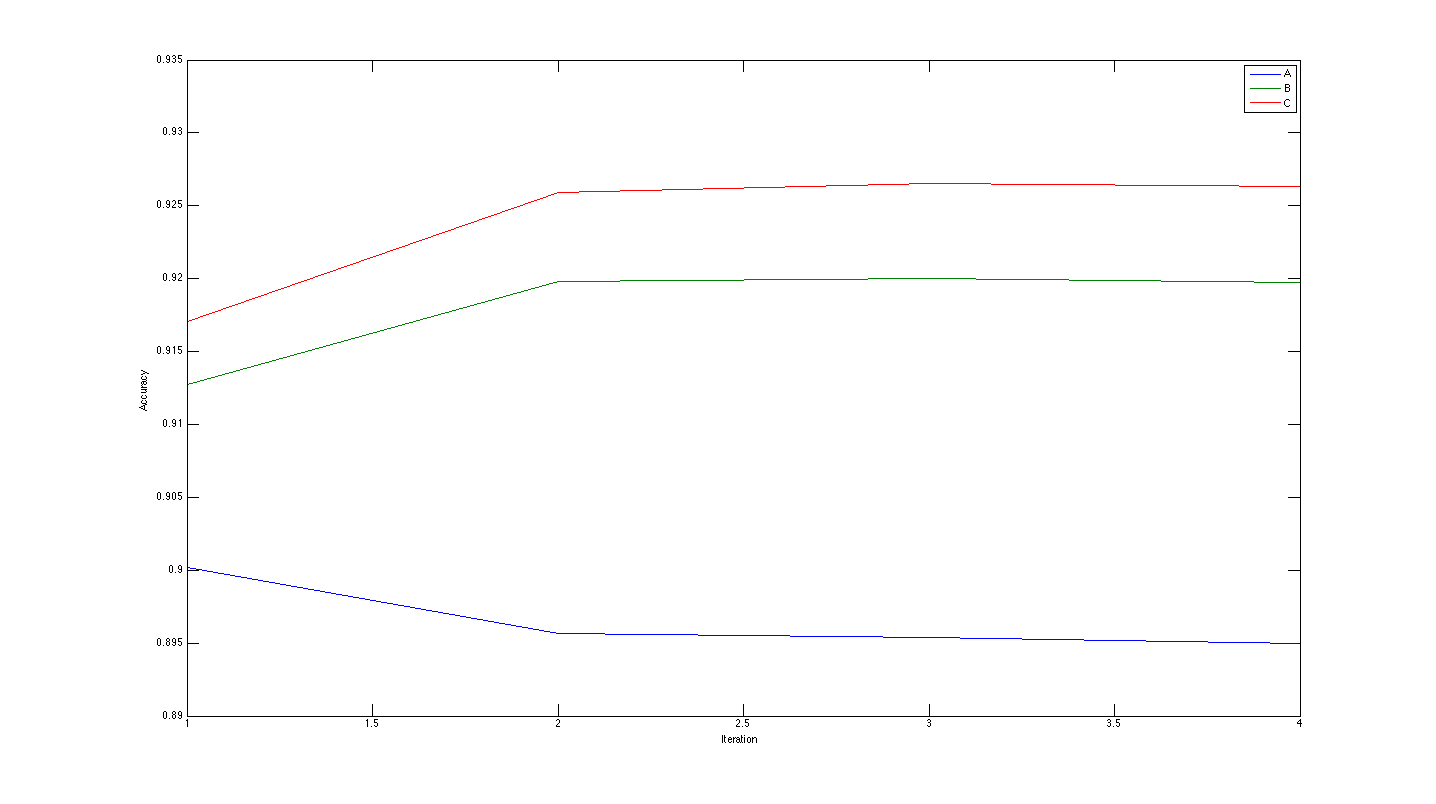
\includegraphics[width=\textwidth]{../images/Task2}\\
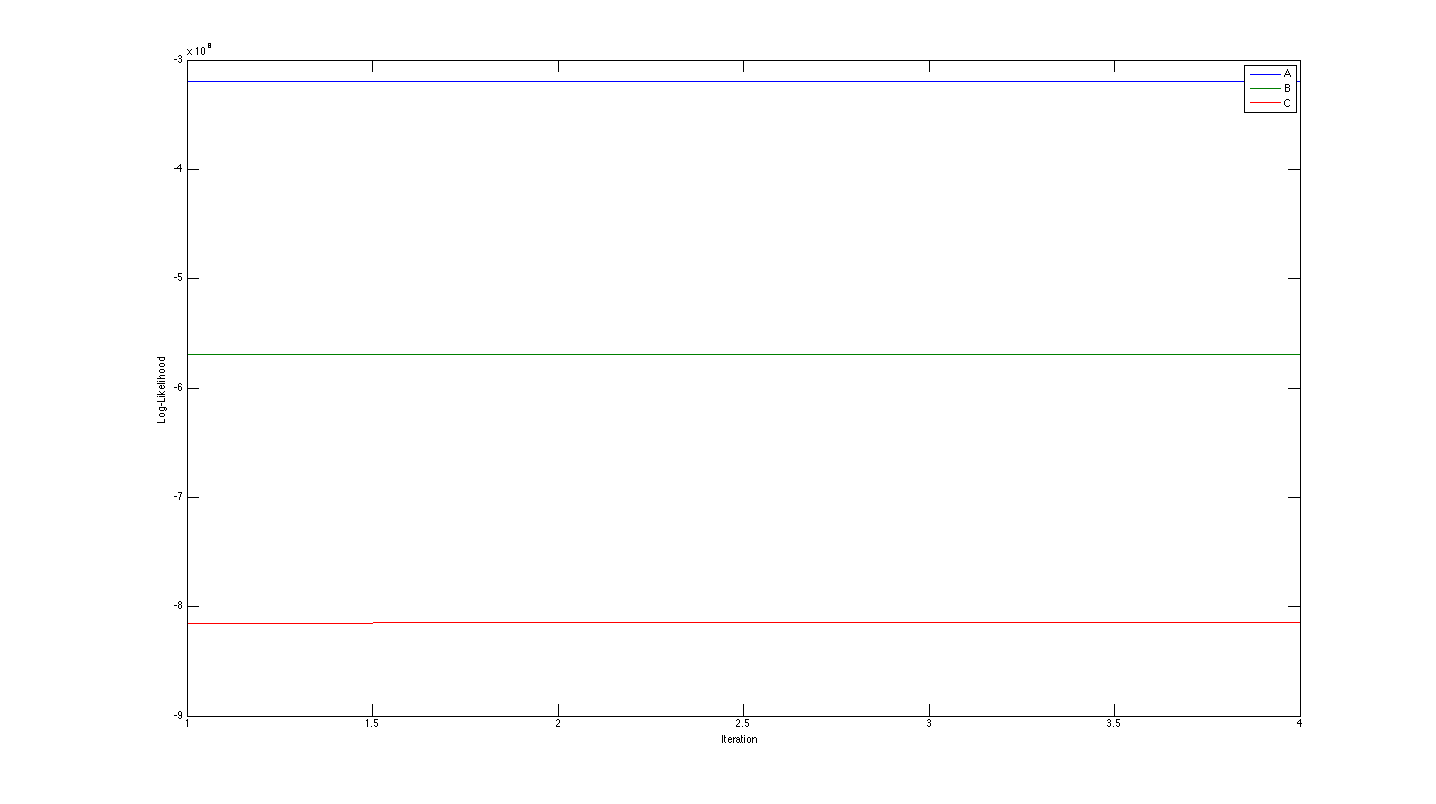
\includegraphics[width=\textwidth]{../images/Task2Log} \\

\newpage

		\item[(c)]
		The accuracy for mostly unlabeled data is significantly worse than the previous two cases. This is because our labeled points may not necessarily be representative of our population. For instance a word $w$ may mostly be used as a noun in the Englsh language, but in the labeled set it was most likely a verb, which skews our results. This is supported by looking at the model accuracy on the labeled points, which are on average even worse that performance on the total data set. Our labeled points were not the best possible choices as a representative sample set. Unlike the previous two cases, we do not see consistent improvement in accuracy by putting the word in context witht he preceeding and following words. We also do not see the same peaking behavior as with the half labeled data set. This is expected because our predictor will take longer to converge near the true clusters when given less initial information. \\
		
\begin{tabular}{ l c r }
Model A & &\\
Model accuracy & on labeled data: 0.701425289901 &\\
Iter 1 & Log-likelihood = -12349648.2363 & Model accuracy: 0.754789250823\\
Iter 2 & Log-likelihood = -12073983.0009 & Model accuracy: 0.754787036781\\
Iter 3 & Log-likelihood = -11975392.0625 & Model accuracy: 0.754618769546\\
Iter 4 & Log-likelihood = -11932227.8478 & Model accuracy: 0.754499211247\\
\end{tabular}\\

\begin{tabular}{ l c r }
Model B & &\\
Model accuracy & on labeled data: 0.720318822129&\\
Iter 1 & Log-likelihood = -22278567.2639 & Model accuracy: 0.71348296571\\
Iter 2 & Log-likelihood = -21614389.7550 & Model accuracy: 0.740204245427\\
Iter 3 & Log-likelihood = -21319755.7617 & Model accuracy: 0.752331663576\\
Iter 4 & Log-likelihood = -21198638.9397 & Model accuracy: 0.753987767415\\
\end{tabular}\\

\begin{tabular}{ l c r }
Model C & &\\
Model accuracy & on labeled data: 0.661033404367&\\
Iter 1 & Log-likelihood = -31965386.5012 & Model accuracy: 0.705529017795\\
Iter 2 & Log-likelihood = -30864290.6209 & Model accuracy: 0.751588852296\\
Iter 3 & Log-likelihood = -30418885.6881 & Model accuracy: 0.768797498132\\
Iter 4 & Log-likelihood = -30247870.7302 & Model accuracy: 0.772801594111\\
\end{tabular}\\
\newpage
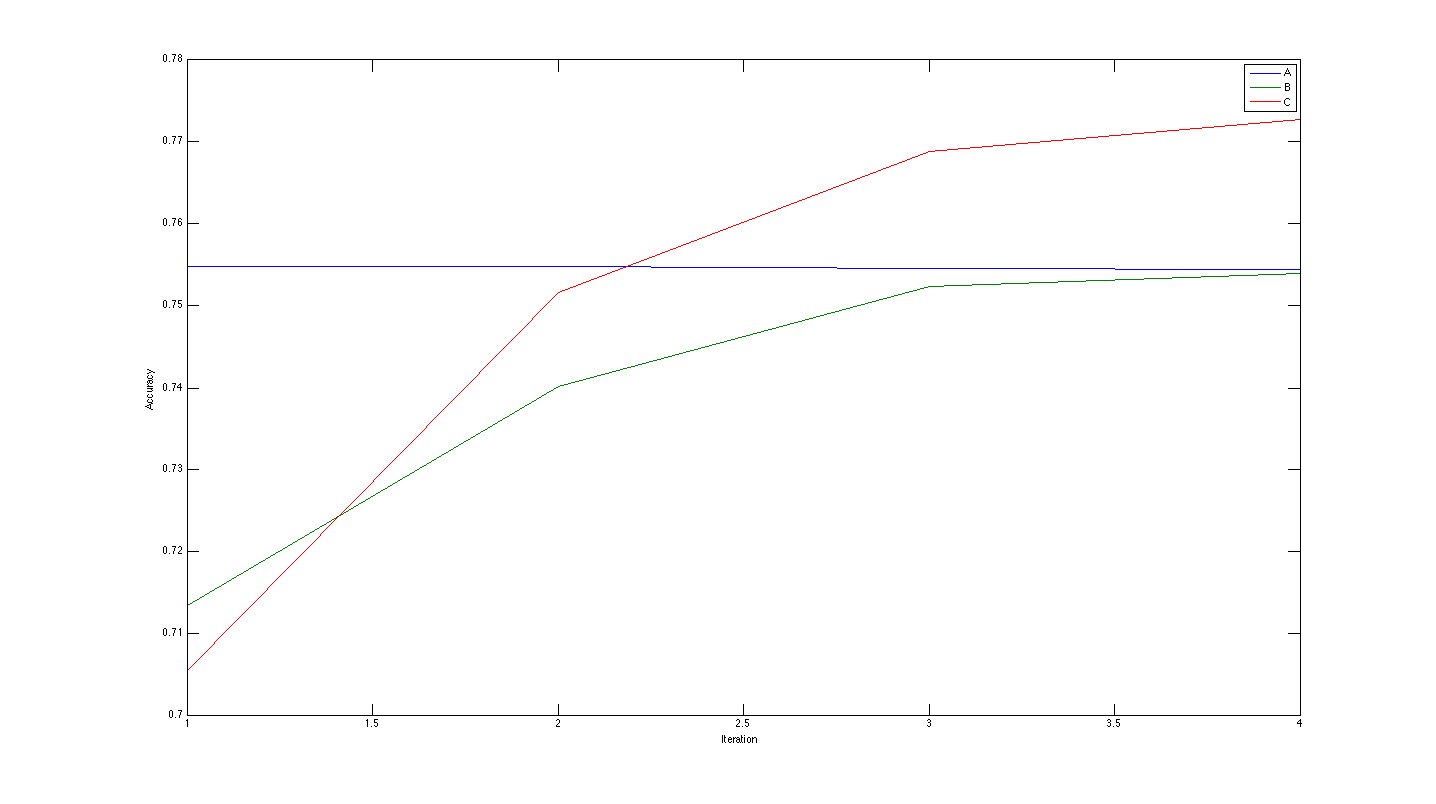
\includegraphics[width=\textwidth]{../images/Task3}\\
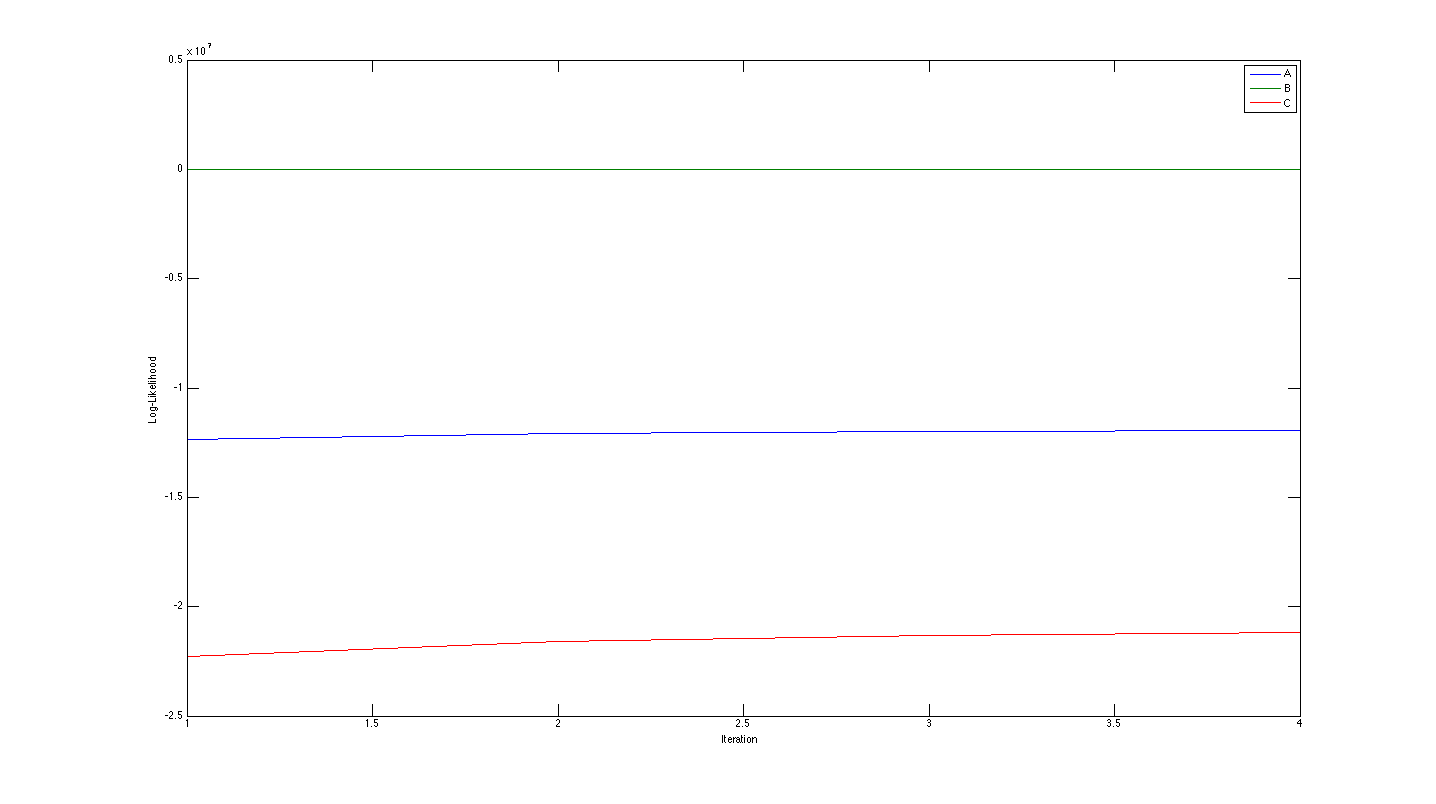
\includegraphics[width=\textwidth]{../images/Task3Log} \\
	\end{enumerate}

\newpage 

\item[5.]
	\begin{enumerate}
	\item[(a)]
		Best word: genes\\
		Probability: 0.99975953723499744\\
		Tag:  'NNS'\\
	\item[(b)]
		Worst word: undercut\\
		
		Foreigners complain that they have limited access to government procurement in Japan, in part because Japanese companies unfairly \texttt{undercut}(VBP)  them.\\
		For Nekoosa, defense options may be \texttt{undercut} (JJ) somewhat by the precarious state of the junk-bond market, which limits how much value the target could reach in a debt-financed recapitalization.\\
		Japan's biggest computer maker last week \texttt{undercut} (VBD) seven competitors to win a contract  to design a mapping system for the city of Hiroshima 's waterworks.\\
	\end{enumerate}
	
	Code for fiding best/worst predictors below (best changes the code below to greater than rather than less than and best starts at 0 instead of 100). Respectively found words with highest and lowest prediction accuracy for tags.\\

\begin{lstlisting}   
def predictA(wordList, pt, ptw, ptpw, ptnw, tags, voc):
	# (prediction %, tag, word)
	best  = (100, None, None)
	mahTags = dict (zip(tags.values(),tags.keys()))
	wurds = dict (zip(voc.values(),voc.keys()))
	# pred is the list of prediction, each element is a list of tag index predictions for each word in the sentence
	pred = []
	# Predict tag index in each sentence based on Model A
	for sent in wordList:
		cur_pred = []
		for pos in range(len(sent)):
			pred_tag = (pt * ptw[:,sent[pos]]).argmax(axis=0)
			maxVal = np.amax(pt * ptw[:,sent[pos]], axis=0) / np.sum((pt * ptw[:,sent[pos]]))
			# Word must be alpha chars
			if maxVal < best[0] and re.match('^[\w-]+$', mahTags[pred_tag]) is not None and re.match('^[\w-]+$', wurds[sent[pos]]) is not None:
				best = (maxVal, mahTags[pred_tag], wurds[sent[pos]])
			cur_pred.append(pred_tag)
		pred.append(cur_pred)
	print 'Best', best
	return pred
\end{lstlisting}
\end{enumerate}

\end{document}